\documentclass[UTF8,a4paper,12pt,oneside]{ctexrep}

\usepackage{geometry}
\usepackage{setspace}
\usepackage{booktabs}
\usepackage{longtable}
\usepackage{tabularx}
\usepackage{array}
\usepackage{xurl}
\usepackage{enumitem}
\usepackage{xcolor}
\usepackage{hyperref}
\usepackage{fancyhdr}
\usepackage{titlesec}
\usepackage{float}
\usepackage{graphicx}
\usepackage{listings}
\usepackage{amsmath}
\usepackage{amssymb}
\usepackage{graphicx}
\usepackage{tikz}
\usetikzlibrary{arrows.meta,positioning}
\geometry{left=2.8cm,right=2.8cm,top=2.8cm,bottom=2.8cm}
\onehalfspacing
\setlength{\parindent}{2em}
\setlength{\parskip}{0.30em}
\setlist[itemize]{leftmargin=2.3em,itemsep=0.25em}
\setlist[enumerate]{leftmargin=2.6em,itemsep=0.25em}

\setCJKmainfont{NotoSerifCJKsc-Regular.otf}[
  Path = ./font/,
  BoldFont = NotoSerifCJKsc-Bold.otf
]

\setmonofont{consola.ttf}[
  Path = ./font/,
  BoldFont = consolab.ttf,
  ItalicFont = consolai.ttf,
  BoldItalicFont = consolaz.ttf
]

\hypersetup{
  colorlinks=true,
  linkcolor=black,
  urlcolor=blue,
  citecolor=black,
  pdfauthor={seccomp-privacy-platform team},
  pdftitle={面向电商隐私分析场景的 SSE + PJC 平台设计与实现}
}

\pagestyle{fancy}
\setlength{\headheight}{15pt}
\fancyhf{}
\fancyhead[C]{面向电商隐私分析场景的 SSE + PJC 平台设计与实现}
\fancyfoot[C]{\thepage}
\renewcommand{\headrulewidth}{0.4pt}

\ctexset{
  chapter = {
    name = {第,章},
    number = \chinese{chapter},
    format = \centering\zihao{3}\heiti,
    beforeskip = 12pt,
    afterskip = 18pt
  },
  section = {
    format = \zihao{4}\heiti,
    beforeskip = 12pt,
    afterskip = 6pt
  },
  subsection = {
    format = \zihao{-4}\heiti,
    beforeskip = 8pt,
    afterskip = 4pt
  }
}

\lstset{
  basicstyle=\ttfamily\small,
  breaklines=true,
  frame=single,
  columns=fullflexible,
  keepspaces=true,
  backgroundcolor=\color{gray!5}
}

\newcommand{\project}{seccomp-privacy-platform}
\newcommand{\pipeline}{metadata/control-plane $\rightarrow$ SSE $\rightarrow$ recovery $\rightarrow$ bridge $\rightarrow$ PJC $\rightarrow$ release}
\newcommand{\filepath}[1]{\path{#1}}
\newcommand{\figplaceholder}[2]{
  \begin{figure}[H]
    \centering
    \fbox{
      \begin{minipage}[c][0.28\textheight][c]{0.86\textwidth}
        \centering
        \vspace{0.6em}
        {\heiti 待补充图片}\\[0.8em]
        #1\\[0.8em]
        {\small 建议使用白色或浅色背景，避免大面积红色、黑色和强烈渐变。}
        \vspace{0.6em}
      \end{minipage}
    }
    \caption{#2}
  \end{figure}
}

\begin{document}

\begin{titlepage}
  \centering
  \vspace*{1.5cm}
  {\zihao{2}\heiti 面向电商隐私分析场景的\\[0.3em]SSE + PJC 平台设计与实现\par}
  \vspace{2.8cm}
  {\zihao{3}\bfseries 项目结题报告\par}
  \vspace{4.8cm}
  \begin{tabular}{>{\bfseries}r l}
    作品名称： & 面向电商隐私分析场景的 SSE + PJC 平台 \\
    项目仓库： & \project \\
    作者： & 张宇杰、屈鸣成、张隽瑄 \\
    指导教师： & 付仕辉 \\
    学校/学院： & 山东大学网络空间安全学院 \\
    日期： & \today \\
  \end{tabular}
  \vfill
\end{titlepage}

\pagenumbering{Roman}

\chapter*{摘要}
\addcontentsline{toc}{chapter}{摘要}

电商平台、广告平台、支付服务商、物流服务商和风控团队在实际业务中分别掌握不同类型的数据。广告侧掌握曝光和点击，电商侧掌握订单和复购，支付侧掌握交易状态，物流侧掌握履约节点，客服系统掌握售后与投诉记录。这些数据联合起来能够回答广告归因、复购分析、风险名单交集、客服回访和合规审计等问题；但如果直接交换邮箱、手机号、设备标识、订单金额和用户行为链路，又会造成明显的隐私泄露与合规风险。

本项目围绕这一矛盾，设计并实现了一个面向电商隐私分析场景的 SSE + PJC 隐私计算平台。系统以控制面数据库记录租户、数据集、调用方、权限、策略和工作流状态；以可搜索对称加密（Searchable Symmetric Encryption，SSE）完成加密数据上的候选筛选；以受控记录恢复服务在授权范围内恢复最小必要字段；以 Rust Bridge 完成 join key 规范化、作用域 HMAC 令牌化、PJC 输入生成和输入承诺；最后接入 Google Private Join and Compute（PJC）完成两方交集统计和交集值求和，并通过 release gate、隐私预算、审批流、source attestation、audit chain 和 external anchor 控制最终结果发布。

结题时，项目已经完成 \pipeline{} 端到端主链路。标准示例得到交集数量 2、交集金额 425；Rust Bridge 在百万级双方输入下完成准备约 4.437 秒；流式 PJC 路径完成百万级双方输入计算；record recovery、Bridge、PJC、release、metadata sidecar、operator console、schema gate、负向安全测试和 benchmark 均形成了可运行入口和结构化证据。项目不只是把两个密码库拼接起来，而是将候选筛选、明文恢复边界、跨方计算、结果发布和审计验证组织为一条可治理的工程链路。

本项目的创新点主要体现在系统组合和工程治理层面。现有 SSE、PSI/PJC、数据净室和联邦学习框架已经提供了重要基础，但单个协议无法回答真实场景中的任务审批、输入来源、发布边界、重复查询、审计归档和故障证据问题。本项目在电商隐私分析场景中补齐了这些协议外治理环节，形成了可复现、可验证、可展示的平台基线。同时，项目也明确保留边界：当前 PJC 仍属于半诚实参与方模型，SSE 仍存在搜索模式和访问模式泄露，真实身份根、KMS、不可变审计锚点和高可用数据库仍需要在目标生产环境长期运行。

\vspace{1em}
\noindent\textbf{关键词：} 可搜索加密；Private Join and Compute；隐私计算；电商分析；审计治理；隐私预算；数据净室

\tableofcontents
\clearpage
\pagenumbering{arabic}

\chapter{作品概述}

\section{背景分析}

随着电子商务和数字广告业务不断发展，广告平台、电商平台和风控机构之间的数据协同需求日益增加。例如，广告平台需要结合电商平台的订单数据评估投放效果，电商平台也可能需要与外部风险名单进行匹配。然而，这类跨平台分析通常涉及邮箱、手机号、设备标识和订单金额等敏感信息，直接交换明文数据容易造成用户身份泄露和跨平台画像关联。因此，如何在保护原始数据的前提下完成查询、匹配与聚合，已成为隐私计算领域的重要研究问题。

\subsection{可搜索加密的发展现状}

传统加密能够保护数据的存储安全，但加密后的数据通常无法直接检索。若每次查询都需要先解密全部数据，不仅效率较低，也会增加明文暴露风险。

可搜索加密技术允许服务器在不了解数据明文和查询内容的情况下，根据查询令牌在密文数据中完成检索。其中，可搜索对称加密具有计算效率较高、适合大规模数据处理等特点，已被应用于加密数据库和云存储等场景。

目前，可搜索加密已经能够支持关键词查询、布尔查询和动态更新等功能，但通常仍会泄露查询次数、访问位置和结果规模等信息。因此，在实际应用中，还需要通过查询限制和访问控制降低访问模式泄露带来的风险。

\subsection{数据规范化与令牌化的发展现状}

跨平台数据通常存在格式不一致的问题。例如，同一个邮箱可能存在大小写差异，手机号也可能包含国家区号、空格或连接符。若不进行统一处理，同一用户在不同平台中的记录可能无法正确匹配。

数据规范化可以统一邮箱、手机号等关联字段的表示形式。在此基础上，通常还需要使用哈希或令牌化技术隐藏原始标识。与普通哈希相比，HMAC 等带密钥哈希算法能够降低邮箱和手机号被字典枚举恢复的风险。

为了避免不同任务之间的用户标识被长期关联，令牌化过程还需要限制密钥的使用范围，并针对不同任务、数据集或业务范围生成相互隔离的令牌。

\subsection{隐私集合计算的发展现状}

隐私集合求交允许两个参与方在不公开各自完整数据集合的情况下，计算双方共有的元素。该技术可以应用于广告归因、联合风控、黑名单匹配和跨平台用户统计等场景。

随着相关研究的发展，隐私集合计算已经不再局限于获得交集元素，还可以进一步统计交集数量，或者对交集元素对应的金额、次数等数值进行聚合。Private Join and Compute 等技术便能够在保护非交集数据的同时，完成用户匹配和交集值求和。

不过，隐私集合计算主要保护协议执行过程，并不能单独解决输入数据规范化、重复查询和小样本结果泄露等问题。因此，它通常需要与令牌化、查询控制和结果发布策略结合使用。

\subsection{结果治理与审计的发展现状}

隐私计算协议可以降低原始数据在计算过程中的暴露风险，但最终输出的统计结果仍可能泄露敏感信息。例如，当交集人数过少时，交集金额可能直接反映某个特定用户的行为；反复执行条件相近的查询，也可能通过结果差异推断个体是否存在。

因此，隐私计算系统通常需要设置最小交集规模、查询频率限制和重复查询检测等发布规则，避免过细结果被直接公开。同时，还需要记录查询发起者、使用的数据范围、计算结果和策略判断过程，以便对整个数据处理流程进行追踪和复核。

结构化审计日志、哈希链和数字签名等技术可以增强审计记录的完整性，使历史记录被修改或删除时能够被及时发现。通过将密码学计算与结果治理、访问控制和审计机制相结合，才能形成较为完整的隐私数据处理体系。

\section{项目问题定义}

本项目面向电商与广告平台之间的跨方数据分析需求，研究如何在不直接交换原始用户标识和业务明细的前提下，使参与方在特定调用者、租户、数据集和业务目的范围内完成交集规模统计与交集值聚合。除计算结果本身外，系统还需要对数据如何进入计算、哪些记录能够被恢复、计算输入是否被替换以及结果是否允许发布作出明确约束，并为整个过程保留可验证、可审计的结构化证据。

第一，进入跨方计算的关联标识必须经过统一处理。邮箱、手机号等原始 join key 不能直接写入 PJC 输入，而应先按照指定规则完成规范化，再结合任务作用域和密钥生成 HMAC-SHA256 令牌。参与双方在使用一致规范化规则、令牌方案、密钥版本和作用域的情况下，可以对同一标识生成可匹配的令牌，同时避免在计算文件中直接暴露原始标识，并降低不同任务之间发生标识关联的风险。

第二，密文检索结果与明文字段访问权限必须相互分离。SSE 阶段仅产生符合检索条件的候选记录标识，这些标识不能被视为读取完整业务记录的授权。后续记录恢复需要由独立服务完成，并对调用者、角色、关联字段、数值字段、过滤条件、候选数量、输出行数以及输入输出路径进行校验。恢复结果仅保留当前计算所需的 join key；当计算方承担数值聚合角色时，再增加被允许的 value 字段，从而控制明文数据的恢复范围。

第三，计算链路中的输入、作业信息和结果必须保持一致。Bridge 在生成 `server.csv` 和 `client.csv` 的同时，需要记录源文件摘要、输出文件摘要、规范化方式、令牌作用域、密钥版本、去重策略和数值字段策略，并将这些信息写入作业元数据和输入承诺文件。PJC 执行结果、双方证据、策略审计记录和公开报告则通过作业标识及 SHA-256 摘要继续关联。在严格发布检查下，只要输入承诺、PJC 结果摘要或相关证据之间出现不一致，结果就不能进入公开发布阶段。

第四，PJC 得到的统计结果不能被直接视为可公开结果。系统需要根据配置检查最小交集规模、差分隐私参数和隐私预算记录，并对重复查询、近似查询、重叠时间窗口、预算耗尽和 bucket 探测等情况作出限制。对于需要人工处理的近似查询，审批结果还必须与对应作用域和查询指纹绑定，并且只能被消费一次。只有发布策略、预算决策和必要证据均满足要求时，计算结果才能通过服务端发布门。

第五，结题成果需要具备可复核性。候选导出、记录恢复、Bridge 输入构造、PJC 执行、结果发布和审计等关键阶段均应产生结构化输出，并通过 JSON Schema 固化其字段与语义。在此基础上，利用 contract check、smoke test、benchmark、审计链与 seal 校验、篡改检测以及 live evidence gate 对系统功能、接口一致性、性能和安全约束进行检查，使项目结论能够由实际代码、运行结果和证据文件共同支撑，而不是仅依赖流程描述。


\section{核心项目工作}

本项目的核心工作围绕一条从密文检索到结果发布的端到端隐私计算链路展开，而非若干独立功能的简单组合。链路首先由 SSE 模块在加密数据上完成候选记录筛选，并依据导出策略限制调用者身份、参与角色、可使用字段以及结果规模。候选记录随后进入独立的记录恢复服务，由该服务在授权范围内恢复计算所必需的字段，从而将密文检索能力与明文字段访问权限分离。

恢复后的必要数据由 Rust Bridge 进一步处理。Bridge 对邮箱、手机号等 join key 进行规范化，并结合任务作用域生成 HMAC-SHA256 令牌，同时形成 PJC 输入、作业元数据和输入承诺。此后，系统调用 Google Private Join and Compute 完成两方集合求交、交集规模统计和交集值聚合。计算结果并不直接对外发布，而是继续经过 release gate、privacy budget、source attestation 和 audit chain 等机制检查，以确认发布条件、输入输出绑定关系及审计证据满足既定要求。

在主链路之外，项目还完善了支撑系统运行的控制面和操作面。Metadata sidecar 集中记录租户、数据集、服务、调用方、策略、密钥、作业、审计和隐私预算等状态；Query workflow 将请求提交、审批、执行、状态回写和结果查看连接起来；Operator dashboard 与 Operator console 则提供作业管理、请求处理、审计查询、数据目录、权限管理、恢复服务状态、可观测性、合规检查和安全状态等功能。通过这些工作，项目在完成隐私计算主流程的同时，也形成了相应的管理、验证和展示能力。

\begin{longtable}{p{0.27\textwidth}p{0.62\textwidth}}
\caption{核心项目工作}\\
\toprule
\textbf{工作方向} & \textbf{完成内容} \\
\midrule
\endfirsthead
\toprule
\textbf{工作方向} & \textbf{完成内容} \\
\midrule
\endhead
\bottomrule
\endfoot
SSE 候选筛选 & 在加密记录和加密索引上返回候选记录标识，保留 candidate selection 能力，并通过 export policy 限制 caller、role、join key、value field、filter field 和最大行数。 \\
受控记录恢复 & 将敏感字段恢复拆成独立服务边界，支持 subprocess、Unix socket、HTTP、mTLS、请求签名、防重放、限流、最大行数和服务审计。 \\
Rust Bridge & 实现 email、phone、id 规范化，生成作用域 HMAC-SHA256 token，输出 PJC 输入、job metadata、bridge audit 和 input commitment。 \\
PJC 集成 & 接入 Google Private Join and Compute，支持 server/client 运行、TLS/mTLS、分桶分片、结果合并、输入承诺检查和百万级流式传输路径。 \\
发布治理 & 实现 release gate、threshold、privacy budget、approval workflow、source attestation、release governance report、audit chain、audit seal 和 external anchor。 \\
控制面与展示 & 实现 metadata sidecar、query workflow、operator dashboard、operator console、platform health、audit query API 和 public report 展示。 \\
验证体系 & 建立 JSON Schema、schema back-compat、contract smoke、CI smoke、malformed input gate、audit tamper test、benchmark 和 live evidence gate。 \\
\end{longtable}


\section{特色描述}

本项目的主要特色，是将可搜索加密、受控记录恢复和隐私集合计算组织为一条具有明确安全边界的完整链路，而不是仅展示一次独立的密码学计算。SSE 负责在密文数据中筛选候选记录，record recovery 将明文字段的恢复限制在授权范围内，Rust Bridge 对原始关联标识进行规范化和作用域令牌化，PJC 完成跨方交集统计与交集值聚合，发布门控和审计机制则对结果公开条件及运行过程进行约束。

各模块之间通过统一的 schema、作业元数据、输入承诺和文件摘要建立关联，使一次计算从候选筛选、字段恢复、输入生成到结果发布均能够被追踪和复核。系统不仅给出最终的交集数量和聚合结果，还能够说明任务由谁发起、使用了哪些数据范围、恢复了哪些必要字段、PJC 输入是否保持一致，以及结果为何被允许或拒绝发布。由此，项目将算法实现与权限控制、结果治理和证据验证结合起来，增强了隐私计算流程的工程完整性和可解释性。

\section{应用前景}

本项目所实现的隐私计算链路可用于广告归因、营销效果分析、风险名单匹配和合规审计等跨方数据协作场景。例如，广告平台与电商平台可以在不直接交换完整用户清单和订单明细的情况下，统计广告触达用户中的成交人数及成交金额；风控机构可以对风险集合与业务数据进行交集分析；合规人员则可以根据策略判断和审计证据复核任务的执行与结果发布过程。

当前系统已经具备端到端运行、策略控制、结果治理和证据验证能力，但尚不能等同于完整的商业数据净室或生产级多租户平台。后续可在现有架构基础上接入更完善的身份与密钥管理系统、生产级数据库和任务队列，扩展更多隐私计算后端，并进一步完善真实部署环境中的高可用、密钥托管和外部不可变审计存储。


\chapter{作品设计与实现}

本章从总体设计、关键技术原理和系统实现三个方面，对项目的设计思路与实现过程进行说明:SSE 模块用于缩小候选数据范围，记录恢复服务限制明文字段的读取，Rust Bridge 隔离原始关联标识，PJC 完成跨方交集统计与聚合计算，发布门控则决定计算结果能否公开。各阶段通过作业元数据、输入承诺、文件摘要和结构化审计记录建立联系，使系统不仅能够得到计算结果，还能够说明结果的产生过程及其发布依据。

\section{总体设计}

\subsection{设计目标}

本项目面向电商平台与广告方之间的跨方数据协作场景。广告方通常掌握用户曝光、点击和营销触达等信息，电商平台则保存订单、交易和会员数据。双方希望统计广告触达用户中的成交人数及成交金额，但又不能直接交换邮箱、手机号、用户标识和订单明细。

若将双方数据集中到同一服务中进行明文计算，计算方将能够接触完整用户清单；若只对邮箱和手机号进行普通哈希，则仍可能受到字典枚举和跨任务关联攻击；若仅运行隐私集合计算协议，而不限制协议前的数据恢复和协议后的结果发布，也可能通过中间明文、小规模交集或重复查询推断个体信息。

因此，本项目的设计目标不仅是完成两方集合的交集统计和交集值聚合，还需要对数据进入计算的方式、明文字段的恢复范围、中间文件的完整性以及最终结果的发布条件进行约束。系统整体遵循最小披露、边界分离、失败关闭和全过程可审计等设计原则。

\textbf{最小披露原则}要求每个阶段只接收完成当前任务所需的数据。SSE 阶段只返回候选记录标识，记录恢复阶段只输出必要的关联字段和数值字段，公开报告只保留经过策略允许的聚合结果。

\textbf{边界分离原则}要求检索、恢复、令牌化、隐私计算和结果发布由不同模块承担。候选记录标识不能直接等同于明文字段读取权限，PJC 计算结果也不能直接等同于可公开结果。

\textbf{失败关闭原则}要求系统在策略、作用域、输入承诺、隐私预算或必要证据缺失时拒绝继续执行，而不是默认放行。

\textbf{全过程可审计原则}要求各阶段产生结构化证据，并通过统一的作业标识和文件摘要将一次任务的输入、执行过程和输出结果关联起来。

\subsection{总体架构}

系统总体架构如图~\ref{fig:overall-architecture} 所示。整个系统由参与方与数据输入、隐私计算主链路、输出与应用、控制面与编排支撑，以及安全审计与观测五部分组成。

\begin{figure}[H]
  \centering
  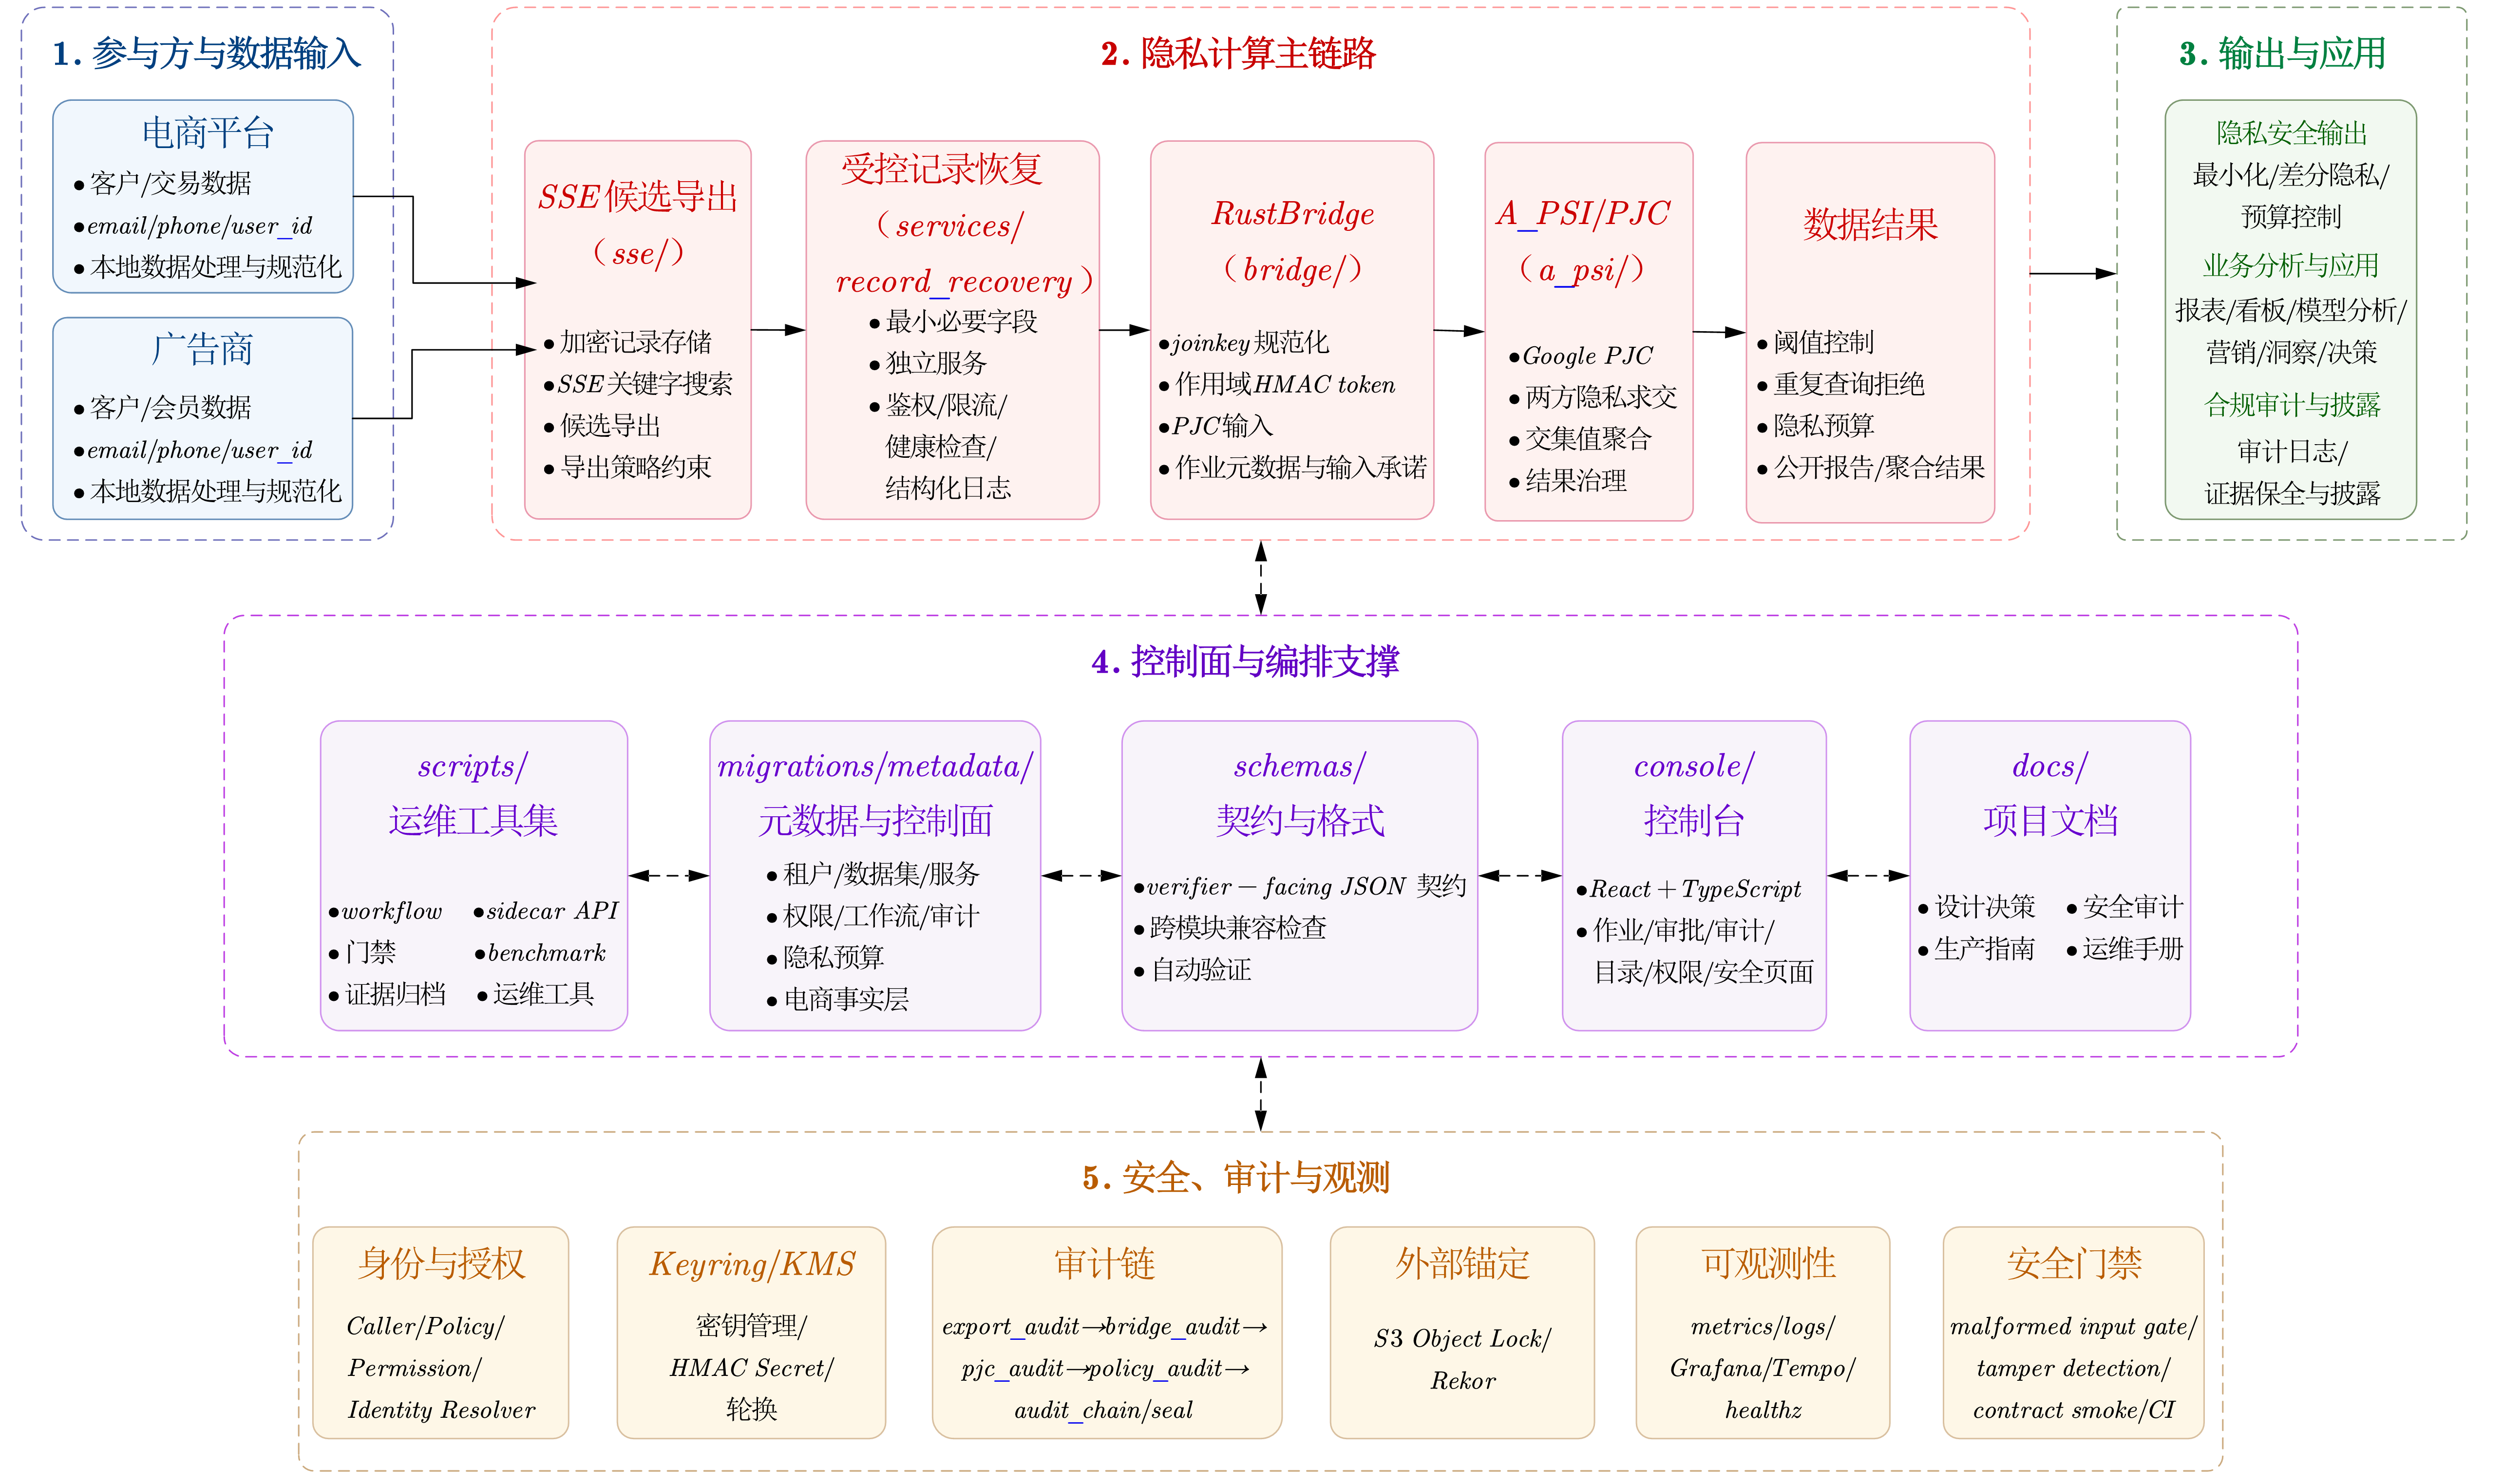
\includegraphics[width=\textwidth]{信安赛.png}
  \caption{面向电商隐私分析场景的 SSE + PJC 平台总体架构}
  \label{fig:overall-architecture}
\end{figure}

参与方主要包括电商平台和广告方。双方分别在本地持有客户、会员、订单或营销触达数据，并选取 email、phone 或 user\_id 等字段作为跨方关联依据。在进入主链路之前，各参与方先在本地完成数据格式整理和必要预处理，不直接交换完整明文数据。

隐私计算主链路是系统的核心。SSE 模块首先在加密索引上执行关键词检索，筛选出可能参与当前任务的候选记录；记录恢复服务根据候选标识和授权策略，仅恢复本次计算所需的字段；Rust Bridge 对恢复后的关联标识进行规范化和作用域 HMAC 令牌化，生成 PJC 输入及相关元数据；A\_PSI/PJC 模块在令牌集合上完成两方交集统计和交集值聚合；计算结果最后进入发布治理阶段，由阈值、重复查询检测、隐私预算和发布策略决定是否生成公开报告。

控制面与编排支撑贯穿整个处理过程。Metadata Sidecar 保存租户、数据集、服务、调用方、策略、作业和隐私预算等状态，Query Workflow 将请求提交、审批、执行和状态回写连接起来，Operator Console 则提供作业、审计、目录、权限和安全状态等页面。

安全、审计与观测模块为主链路提供支撑。身份与授权机制限制调用主体和数据范围，Keyring/KMS 相关接口管理 HMAC secret 和服务凭据，审计链与密封机制记录并验证各阶段证据，外部锚定用于增强审计结果的不可篡改性，可观测性和安全门禁则负责运行状态检查、异常输入检测和契约验证。

\subsection{系统工作流程}

一次完整的跨方隐私分析任务如图~\ref{stream}所示过程执行。


\begin{figure}[H]
  \centering
  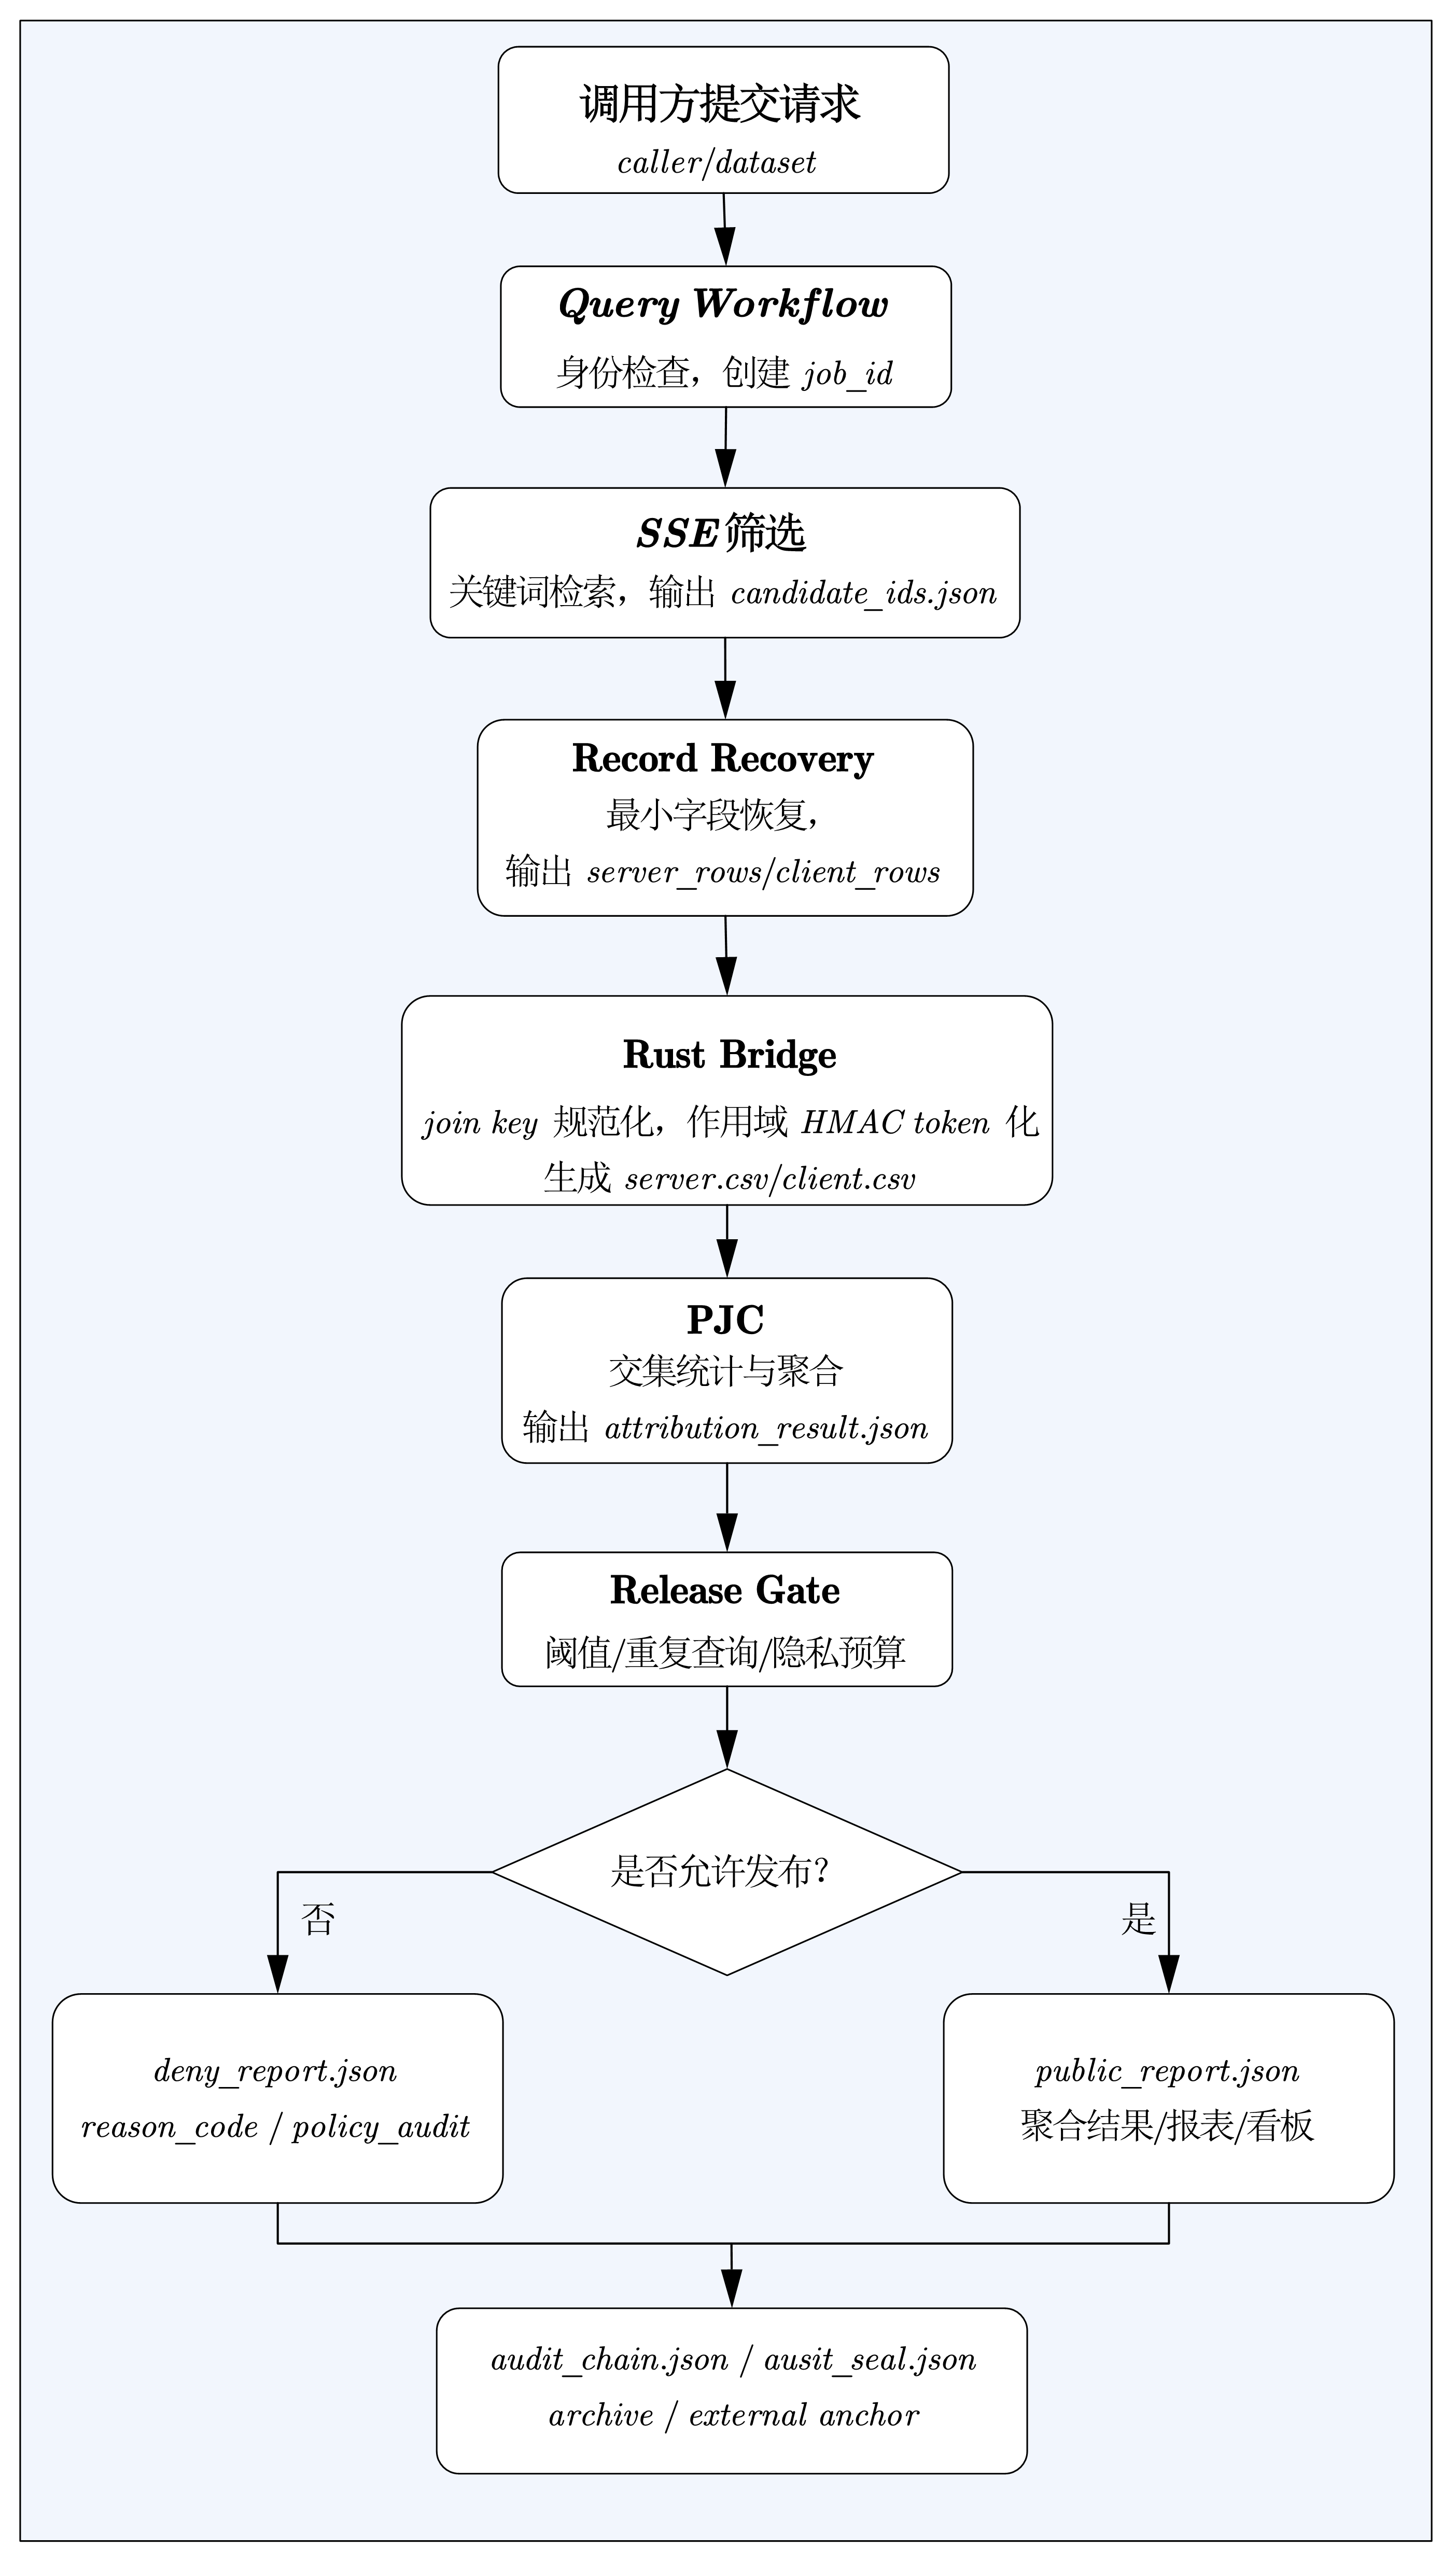
\includegraphics[width=0.6\textwidth]{stream.png}
  \caption{端到端隐私计算任务流程}
  \label{stream}
\end{figure}

首先，调用方提交查询请求，并指定参与任务的数据集、关联字段、数值字段、过滤条件、调用身份、任务作用域和结果发布参数。系统根据调用者身份和数据作用域检查请求是否具有执行资格。

随后，SSE 模块根据检索关键词在加密索引上完成候选筛选，得到候选记录标识集合。该集合只表示哪些记录可能与当前任务相关，并不表示调用方已经获得这些记录的明文读取权限。

候选标识进入记录恢复服务后，服务会再次检查调用方、参与角色、字段范围、过滤条件、候选数量以及输入输出路径。只有满足策略要求的记录才能被解密，并且恢复结果仅保留后续计算所需的最小字段。

恢复后的数据由 Rust Bridge 继续处理。Bridge 对关联标识执行统一规范化，并结合任务作用域生成 HMAC-SHA256 token。随后，Bridge 生成 server 侧和 client 侧的 PJC 输入文件，同时记录作业元数据、输入文件摘要和输入承诺。

PJC 模块使用双方生成的 token 集合执行隐私集合计算，得到交集规模和交集值之和。该结果属于内部计算结果，尚不能直接向业务方公开。

最后，结果进入发布治理阶段。系统依据最小交集阈值、重复查询、隐私预算、审批状态和证据绑定关系判断结果能否发布。允许发布时生成公开报告；拒绝发布时仅记录决策和原因，不公开受限制的聚合结果。

\section{关键技术原理}

本项目使用了 SSEPy 和 Google Private Join and Compute 等开源实现。因此，本节重点说明与本项目主链路直接相关的核心原理。

\subsection{可搜索加密与候选筛选}

传统加密可以保护数据内容，但加密后通常无法直接根据关键词检索。可搜索对称加密允许数据拥有者在加密数据上建立索引，并通过搜索令牌在不直接公开关键词和记录明文的情况下完成查询。

设加密索引为 $\operatorname{EDB}$，关键词 $w$ 对应的搜索令牌为 $\tau_w$，则一次检索过程可以表示为：

\begin{equation}
C_w=\operatorname{Search}(\operatorname{EDB},\tau_w),
\end{equation}

其中，$C_w$ 为与关键词 $w$ 匹配的候选记录标识集合。

本项目主要使用 SSE 的候选筛选能力。SSE 返回的是候选记录标识，而不是完整业务记录。后续记录恢复服务只能围绕集合 $C_w$ 中的候选记录进行处理，并且仍需执行独立的权限检查。通过这种方式，系统将“搜索到某条记录”和“读取该记录的敏感字段”分离开来。

SSE 本身仍可能泄露查询重复关系、访问模式和候选数量。因此，本项目没有将 SSE 描述为完全隐藏查询行为，而是将其作为缩小候选范围和降低明文处理规模的基础技术。

\subsection{加密记录存储与受控恢复}

为了避免候选筛选后直接读取完整明文源文件，项目将业务记录保存到独立的加密记录库中。系统从环境变量中的口令派生 256 位加密密钥：

\begin{equation}
K_{\mathrm{store}}
=
\operatorname{PBKDF2\text{-}HMAC\text{-}SHA256}
(P,s,600000,32),
\end{equation}

其中，$P$ 为记录库口令，$s$ 为随机盐，$600000$ 为迭代次数，$32$ 表示输出 32 字节密钥。

随后，系统使用 AES-256-GCM 对每条记录执行认证加密，并使用带密钥的 HMAC 标签代替原始记录标识。对于记录标识 $id_i$，其查询标签为：

\begin{equation}
tag_i=
\operatorname{HMAC\text{-}SHA256}
(K_{\mathrm{store}},id_i).
\end{equation}

记录库中保存的是标签、随机 nonce 和认证密文，而不是原始记录标识。恢复时，系统根据候选标识重新计算对应标签，只解密标签匹配的记录。

记录恢复服务进一步实现了字段投影。对于 server 角色，只恢复关联字段：

\begin{equation}
\operatorname{Project}_{server}(r)=\{r[join\_key]\}.
\end{equation}

对于需要提供聚合值的 client 角色，则恢复关联字段和被允许的数值字段：

\begin{equation}
\operatorname{Project}_{client}(r)
=
\{r[join\_key],r[value]\}.
\end{equation}

因此，候选记录被解密后并不会将整条业务记录直接交给 Bridge，而是只保留当前 PJC 任务实际需要的数据。

\subsection{关联标识规范化与作用域令牌化}

不同数据源中同一用户的标识可能具有不同表示形式。例如，邮箱可能存在大小写和首尾空格差异，手机号可能包含空格、连接符或不同的国际拨号前缀。若不进行统一处理，同一用户也可能生成不同的匹配值。

设原始关联标识为 $x$，规范化函数为 $N(\cdot)$，则规范化结果为：

\begin{equation}
x'=N(x).
\end{equation}

对于 email，Bridge 会去除首尾空白并转换为 ASCII 小写。对于 phone，Bridge 会去除空格和连接符，保留数字及首位加号，并将国际拨号前缀 \texttt{00} 转换为加号，同时检查号码长度是否符合规范化要求。对于普通 identity 模式，则只去除首尾空白。

规范化完成后，Bridge 使用 token secret 和任务作用域生成 HMAC-SHA256 token：

\begin{equation}
t=
\operatorname{HMAC\text{-}SHA256}
\left(
K_{\mathrm{token}},
x'\parallel\mathrm{LF}\parallel scope
\right),
\end{equation}

其中，$K_{\mathrm{token}}$ 为 token secret，$scope$ 为当前任务的 token scope，$\mathrm{LF}$ 表示换行字节。

将任务作用域写入 HMAC 输入后，同一用户标识在不同任务作用域下会生成不同 token，从而降低跨任务长期关联的风险。PJC 输入文件中只保存生成后的 token，不直接保存原始邮箱、手机号或 user\_id。

\subsection{Private Join and Compute}

完成令牌化后，server 侧和 client 侧分别形成 PJC 输入。设 server 侧 token 集合为：

\begin{equation}
S=\{s_1,s_2,\ldots,s_m\},
\end{equation}

client 侧持有 token 与整数值组成的集合：

\begin{equation}
C=\{(c_1,v_1),(c_2,v_2),\ldots,(c_n,v_n)\}.
\end{equation}

系统需要得到两类结果，即交集规模：

\begin{equation}
N_I=
\left|
S\cap\{c_1,c_2,\ldots,c_n\}
\right|,
\end{equation}

以及交集元素对应值的聚合结果：

\begin{equation}
V_I=
\sum_{c_i\in S}v_i.
\end{equation}

项目接入的 Google Private Join and Compute 使用椭圆曲线可交换加密完成双方集合标识的隐私匹配，并使用 Paillier 加法同态加密保护 client 侧的整数值。

协议执行后，双方能够得到交集规模和交集值之和，但不会直接获得完整的对方集合，也不会公开具体哪些标识位于交集中。

需要注意的是，当前 PJC 开源实现采用半诚实安全模型，即假设参与方按照协议步骤执行，但可能尝试从收到的消息中推断额外信息。协议本身不证明双方输入一定来自真实业务数据，因此本项目另外使用来源声明、审批和审计机制对输入过程进行治理，但这些机制不能替代面向恶意参与者的密码学协议。

\subsection{结果发布治理}

PJC 输出的交集规模和交集值之和属于内部计算结果，不能直接视为公开结果。若交集规模过小，聚合值可能暴露单个或少量用户的行为；若调用方反复执行相近查询，也可能通过结果差异推断用户是否属于交集。

系统首先执行最小交集阈值判断。设交集规模为 $N_I$，最小发布阈值为 $k$，则只有满足

\begin{equation}
N_I\geq k
\end{equation}

时，结果才具备进入公开发布阶段的基本条件。

在此基础上，系统进一步结合重复查询检测、近似查询检查、隐私预算和审批状态进行判断。对于同一调用方、数据集和业务目的，系统记录历史查询及预算消耗。当预算耗尽、查询完全重复或时间窗口高度重叠时，结果将被拒绝发布或进入审批流程。

因此，系统将 PJC 和发布门控划分为两个不同阶段：PJC 负责判断结果能否被计算，Release Gate 负责判断结果能否被公开。

\subsection{输入承诺与审计完整性}

为避免 Bridge 输出、PJC 输入和最终报告之间出现中间文件替换，系统会为关键文件计算 SHA-256 摘要。对于任意关键文件 $F$，其摘要表示为：

\begin{equation}
h_F=\operatorname{SHA256}(F).
\end{equation}

Bridge 会记录源输入、\texttt{server.csv}、\texttt{client.csv} 和输入承诺文件的摘要。后续 PJC 和发布阶段重新计算这些摘要，并与作业元数据中记录的值进行比较。

各阶段产生的审计记录最终被汇总为 \texttt{audit\_chain.json}，系统再计算其摘要并生成审计密封：

\begin{equation}
\sigma_{\mathrm{seal}}
=
\operatorname{HMAC\text{-}SHA256}
\left(
K_{\mathrm{seal}},
\operatorname{SHA256}
(\texttt{audit\_chain.json})
\right).
\end{equation}

若审计链文件在生成密封后被修改，其 SHA-256 摘要将发生变化，从而导致密封验证失败。该机制用于检测审计证据在归档和复核过程中的篡改。

\section{系统实现}

\subsection{参与方与数据输入}

系统面向电商平台和广告方两类典型参与方。电商平台侧主要提供订单、交易和会员数据，广告方侧主要提供广告触达、点击和客户数据。双方在本地选择 email、phone 或 user\_id 等字段作为关联依据，并完成字段整理和数据预处理。

输入阶段不要求参与方直接上传完整数据集，而是要求明确当前任务使用的数据集、关联字段、数值字段和过滤条件。通过这种方式，后续各模块可以围绕固定的数据作用域执行权限检查，并减少与当前任务无关的数据进入隐私计算链路。

\subsection{SSE 候选导出}

SSE 模块基于 SSEPy 原型进行扩展。该模块保留了加密索引构建、单关键词查询、多关键词关联、数据更新和删除等能力。在本项目主链路中，SSE 主要承担候选记录筛选任务。

执行查询时，系统首先根据指定关键词向 SSE 服务提交搜索令牌，获得匹配的候选记录标识。随后，候选导出程序根据这些标识筛选本地数据或加密记录库中的记录。

候选导出并非无条件执行，而是需要经过 export policy 检查。策略可以限制 caller、role、join key 字段、value 字段、过滤字段、过滤值、候选数量和最大输出行数。若请求超出授权范围，系统将拒绝导出，并在审计记录中写入对应的 decision 和 reason code。

SSE 导出审计会记录候选来源、候选数量、过滤条件摘要和输出文件摘要，但不记录原始 join key、原始过滤值或敏感密钥。

\subsection{受控记录恢复}

记录恢复模块将候选标识转换为 Bridge 所需的最小字段集合。该模块被设计为独立服务边界，
恢复服务支持 subprocess、Unix socket 和 HTTP 三种调用方式。其中，Unix socket 适合同一主机内的独立服务，HTTP 适合跨进程或跨主机部署，并可进一步配置 TLS 或 mTLS。

恢复请求到达服务后，系统依次执行认证 token 检查、时间戳校验、请求摘要验证、HMAC 请求签名校验和调用者授权。随后检查 role、join key、value 字段、过滤条件、候选数量以及记录库和输出路径。

服务只解密候选标签匹配的记录，并根据角色执行字段投影。Server 侧只输出 join key，Client 侧输出 join key 和经过授权的 value 字段,最终输出文件的行数和 SHA-256 摘要会被记录到结构化服务审计中。

这种设计将 SSE 查询和明文恢复分离开来。即使调用方获得了候选 ID，也不能绕过恢复服务读取完整业务记录。

\subsection{Rust Bridge}

Bridge 使用 Rust 实现并编译为单一可执行文件。其主要任务是将恢复后的业务字段转换为 PJC 可以直接使用的输入格式。

Bridge 支持 CSV 和 JSONL 两种输入格式。执行过程中，它首先读取 join key 和可选的 value 字段，然后根据配置执行 identity、email 或 phone 规范化。规范化结果进一步结合 token secret 和 token scope 生成 HMAC-SHA256 token。

Server 侧输出文件 \texttt{server.csv} 每行只包含一个去重后的 token；Client 侧输出文件 \texttt{client.csv} 每行包含一个 token 及其对应整数值。

对于重复 token，当前默认去重策略为保留最大值，即：

\begin{equation}
V(t)=\max\{v_i\mid t_i=t\}.
\end{equation}

Bridge 还会根据 value policy 检查数值字段白名单、最小值、最大值、是否允许负数、数值单位和货币代码。生产模式下，整数聚合需要显式配置最大值、允许字段和数值单位。

除 PJC 输入文件外，Bridge 还会生成：

\begin{itemize}
  \item \texttt{job\_meta.json}，记录任务参数、规则版本、文件路径和行数；
  \item \texttt{input\_commitments.json}，记录源文件和输出文件摘要；
  \item \texttt{bridge\_audit.jsonl}，记录执行结果、摘要和运行时间。
\end{itemize}

生产模式禁止直接通过命令行参数传递 token secret，只允许从环境变量或外部密钥适配器获取，避免密钥出现在命令历史和进程参数中。

\subsection{PSI/PJC 集成}

PJC 相关实现保留了 Google Private Join and Compute 的核心部分，并在其外层增加作业校验、运行脚本、TLS 配置、结果整理和审计证据生成。
PJC 启动前，系统首先检查 Bridge 生成的作业元数据，确认 token scheme、token scope、密钥版本、规范化规则和输入文件均符合要求，同时检查 CSV 实际行数是否与元数据记录一致。

项目支持单机和双机两种运行方式。单机模式在本地同时启动 server 和 client，适合演示和测试；双机模式允许双方分别在不同主机运行，并通过 TLS 或 mTLS 建立通信。

针对较大规模输入，项目还提供了分桶、分片和流式传输路径。分桶和分片用于将完整任务拆分为多个较小 PJC 作业，最后根据 manifest 合并交集数量和交集值；流式传输用于降低超大单条 gRPC 消息带来的内存和消息大小限制。

PJC 最终产生的核心结果为：

\begin{equation}
\texttt{intersection\_size}=N_I,
\qquad
\texttt{intersection\_sum}=V_I.
\end{equation}

该结果属于内部结果，需要继续进入发布治理阶段。

\subsection{结果发布治理}

结果治理主要由 \texttt{policy\_release.py} 和服务端 Release Gate 完成。

\texttt{policy\_release.py} 读取 PJC 结果后，依次执行调用者检查、查询频率检查、重复查询检测、最小交集阈值判断、隐私预算检查和可选差分隐私处理，随后生成 operator report、public report 和 policy audit。

服务端 Release Gate 作为独立于命令行参数的最终发布边界，会再次检查公开报告是否满足策略。严格配置下，发布门可以要求：

\begin{itemize}
  \item 报告中的交集阈值不得低于配置值；
  \item 必须存在当前任务对应的隐私预算允许记录；
  \item 被判定为重复或近似查询的任务不能直接发布；
  \item 公开报告不得包含仅供操作人员使用的内部字段；
  \item PJC 双方证据中的结果摘要必须与策略审计一致；
  \item 输入承诺、来源声明和公开报告之间必须保持一致；
  \item 要求外部锚点时，锚点必须处于实际上传状态。
\end{itemize}

当任一检查失败时，系统生成 deny 决策和对应原因码，而不是继续公开计算结果。

\subsection{安全、审计与观测}

系统在主链路之外设置了身份授权、密钥管理、审计链、外部锚定、可观测性和安全门禁等支撑机制。

身份与授权机制通过 caller、policy、permission 和 identity resolver 等信息限制操作主体及其可访问的数据范围。恢复服务和发布治理阶段都会根据调用身份和作用域重新执行权限检查。

密钥管理部分用于管理 HMAC secret、服务 token 和审计密封密钥。敏感凭据不会被写入业务审计，审计中只保留密钥来源类型和版本信息。

审计链会汇总 SSE export、record recovery、Bridge、PJC 和 policy release 等阶段的结构化记录。系统进一步为审计链生成 seal，并通过归档工具检查文件摘要、HMAC、作业标识和租户作用域。

外部锚定支持将审计摘要写入 S3 Object Lock 或 Sigstore Rekor 等外部存储。严格模式下，本地文件或 planned 状态不能被视为完成外部锚定。

可观测性部分提供健康检查、metrics、日志和 Grafana/Tempo 等适配。安全门禁则通过 malformed input gate、audit tamper test、contract smoke、CI smoke 和 live evidence gate 等方式检查异常输入、审计篡改和跨模块契约错误。







\chapter{项目完成情况与成果}

\section{总体完成情况}

结题时，项目已经由最初的算法衔接原型发展为具有完整处理链路和配套治理能力的隐私计算平台基线。系统不仅能够依次完成 SSE 候选筛选、受控记录恢复、关联标识令牌化、PJC 交集计算和结果发布，还建立了与主链路相配套的任务管理、策略控制、证据验证和操作展示能力。各阶段的运行状态、输入输出摘要和策略决策均能够以结构化形式记录，并由自动化工具进行检查。

因此，项目成果不宜简单概括为“实现了 SSE 和 PJC”。更准确地说，本项目完成了一条面向电商隐私分析场景、包含数据处理链路、控制面、治理面和验证体系的执行流程。该流程已经能够在项目规定的本地和受控部署范围内稳定运行，但仍保留从比赛版平台基线向生产级隐私计算系统演进所需的安全与运维边界。

\begin{longtable}{p{0.22\textwidth}p{0.22\textwidth}p{0.44\textwidth}}
\caption{项目目标与完成情况}\label{tab:goal-completion}\\
\toprule
\textbf{原始目标} & \textbf{完成状态} & \textbf{完成说明} \\
\midrule
\endfirsthead
\toprule
\textbf{原始目标} & \textbf{完成状态} & \textbf{完成说明} \\
\midrule
\endhead
\bottomrule
\endfoot

候选筛选 &
项目范围内完成 &
基于 SSE 实现密文候选记录筛选，并通过 export policy 对调用方、角色、字段、过滤条件和导出规模进行约束，同时记录候选数量、输出摘要和导出审计。 \\

记录恢复 &
项目范围内完成 &
将敏感记录恢复划分为独立服务边界，支持 subprocess、Unix socket 和 HTTP 等调用方式，并实现鉴权、请求签名、时间戳校验、限流、最大行数控制、健康检查和结构化审计。 \\

跨方计算 &
项目范围内完成 &
接入 Google Private Join and Compute，实现两方集合交集规模统计和交集值求和，并扩展分桶、分片及流式传输路径，以支持更大规模输入。 \\

标识保护 &
项目范围内完成 &
使用 Rust Bridge 实现 email、phone 和 identity 的规范化，以及作用域 HMAC-SHA256 token 生成，同时输出 PJC 输入、作业元数据、Bridge 审计和输入承诺。 \\

发布治理 &
项目范围内完成 &
实现最小交集阈值、重复与近似查询检查、隐私预算、审批流程、来源声明、服务端 release gate、审计密封和外部锚点适配，使内部计算结果必须经过策略判断后才能公开。 \\

控制面 &
平台基线完成 &
完成 Metadata Sidecar、Query Workflow、Operator Dashboard 和 Operator Console，能够记录并展示租户、数据集、调用方、策略、作业、审批、预算和审计等状态。 \\

验证体系 &
已完成并持续执行 &
建立 JSON Schema、schema back-compat、contract smoke、CI smoke、安全负向测试、benchmark 和 live evidence gate，对主链路及关键治理边界进行自动检查。 \\

生产级安全 &
保留演进边界 &
当前仍采用半诚实 PJC 安全模型。恶意参与方安全、真实企业身份与密钥信任根、生产级高可用、资源隔离、长期 SRE 运维和持续 live evidence 仍属于后续建设范围。 \\

\end{longtable}

\section{主链路成果}

项目首先完成了从候选数据检索到聚合结果发布的端到端主链路。在标准电商归因示例中，系统从双方的本地数据出发，依次执行 SSE 查询、受控记录恢复、Rust Bridge 处理、PJC 计算和发布策略检查，最终得到：

\begin{equation}
\texttt{intersection\_size}=2,
\qquad
\texttt{intersection\_sum}=425.
\end{equation}

该结果表明，双方原始关联标识经过统一规范化和作用域令牌化后，仍能够在 PJC 中形成一致匹配；Client 侧关联值也能够在不公开具体交集成员的情况下完成聚合。发布阶段进一步生成公开报告，从而验证了从数据准备、隐私计算到结果输出的整体正确性。

与仅输出交集数量和聚合值的算法演示不同，本项目在执行过程中同步生成了覆盖各阶段的结构化证据。SSE export audit 记录候选集合的来源、规模和导出决策；record recovery audit 记录恢复请求、授权范围和输出摘要；bridge audit 记录规范化方式、令牌方案和输入输出哈希；PJC audit 记录计算状态和结果摘要；policy audit 则记录发布判断、原因码和策略依据。

这些证据通过统一的 \texttt{job\_id}、\texttt{correlation\_id} 和文件摘要进行关联，并被进一步汇总为 \texttt{audit\_chain.json}。审计链完成密封后，还可以通过验证与归档工具检查其完整性。因此，最终结果不再是缺少上下文的孤立数字，而是一个具有明确输入来源、处理路径、策略依据和审计证据的计算产物。

\section{控制面成果}

随着主链路逐步完善，项目进一步建设了任务管理和操作展示所需的控制面。Metadata Sidecar 用于保存和查询租户、数据集、服务、调用方、权限、策略、密钥版本、作业、审计及隐私预算等元数据。它可以初始化控制面数据库，导入既有运行产物，并根据 job、caller、tenant、dataset、policy 和 permission 等条件查询任务状态。

Query Workflow 将原本分散的脚本调用组织为具有状态变化的任务流程。调用方可以提交 dry-run 或 execute 请求，系统在完成请求规范化、契约检查和权限判断后生成 submission manifest，并记录任务启动、运行、完成或失败等状态。任务完成后，结果路径、审计路径和发布决策会重新写回控制面，使一次隐私计算任务具备较完整的生命周期记录。

Operator Dashboard 和 Operator Console 在此基础上提供面向操作人员的管理界面。控制台能够展示作业、查询请求、审批队列、隐私预算、审计证据、数据目录、权限状态和平台健康信息，并可通过对应接口发起或查看任务。

控制面的建设改变了项目只能依赖命令行脚本运行的状态。虽然它仍属于比赛版平台基线，而不是完整的生产调度系统，但已经能够将任务发起、状态管理、策略审批、结果查看和审计复核连接起来，使项目具备较清晰的平台使用形态。

\section{安全治理成果}

本项目的安全治理围绕数据进入计算、协议输入生成、结果发布和证据归档四个阶段展开，并落实为可执行的工程机制。

在数据输入阶段，SSE 只返回候选记录标识，调用方不能凭借候选标识直接读取完整业务明文。独立的 Record Recovery 服务会重新检查调用身份、数据作用域、候选数量、字段白名单和输出路径，并只恢复当前角色所需的最小字段。

在协议输入阶段，Rust Bridge 不将原始 join key 直接写入 PJC 文件，而是先执行规范化，再结合任务作用域生成 HMAC-SHA256 token。Bridge 同时为生成的 \texttt{server.csv}、\texttt{client.csv} 和相关元数据计算摘要，并形成 input commitment。后续校验会重新检查文件摘要和行数，从而发现 Bridge 输出在进入 PJC 前被单独替换的情况。

在结果治理阶段，PJC 原始结果必须经过最小交集阈值、重复查询、近似查询、隐私预算和审批状态等检查。Source attestation 用于记录数据来源、作用域和签署责任，并与输入承诺及发布报告建立绑定。Release Gate 则作为服务端最终判断边界，防止因操作人员遗漏命令行参数而直接扩大公开范围。

在证据归档阶段，系统将不同模块产生的审计记录汇总为审计链，并使用 SHA-256 和 HMAC seal 检测文件篡改。归档锚点还可以写入本地链式账本，或通过适配器关联 S3 Object Lock、Sigstore Rekor 等外部机制。

这些治理措施提升了项目对越权恢复、明文扩散、中间文件替换、重复查询和本地审计篡改等工程风险的抵抗能力。不过，它们属于协议外治理，并不能将 Google PJC 的半诚实安全模型直接提升为恶意参与方安全模型。明确这一边界能够避免夸大项目安全性，也使当前成果和后续改进方向更加清晰。


\section{性能与规模验证成果}

在完成端到端功能验证的基础上，项目进一步对 SSE Export、Record Recovery、Rust Bridge、PJC 和完整管线进行了规模测试。该部分工作的主要目的，是验证各模块在输入规模扩大后能否保持正确运行，建立可重复的性能基线，并识别主链路中的主要资源开销，而不是对生产环境吞吐能力作出容量承诺。

测试结果表明，系统已经形成从轻量数据准备到大规模隐私计算的分层验证能力。SSE Export 和 Rust Bridge 均完成了百万级输入测试；Record Recovery 完成了并发请求、mTLS 和最大返回行数门禁验证；PJC 除完成十万级常规运行外，还通过流式传输路径完成了百万级双方输入计算；完整管线则在扩大后的输入规模下保持了结果正确性和证据完整性。

\begin{longtable}{p{0.27\textwidth}p{0.61\textwidth}}
\caption{性能与规模验证代表性结果}
\label{tab:performance-scale-results}\\
\toprule
\textbf{验证对象} & \textbf{代表性结果} \\
\midrule
\endfirsthead
\toprule
\textbf{验证对象} & \textbf{代表性结果} \\
\midrule
\endhead
\bottomrule
\endfoot

标准端到端示例 &
完整执行 SSE、Record Recovery、Rust Bridge、PJC 和 Release 流程，得到
\texttt{intersection\_size=2} 和
\texttt{intersection\_sum=425}，结果与预期一致。 \\

顶层验证闭环 &
16 个 verifier-facing 模块均达到
\texttt{status=ok}、\texttt{repo\_side\_status=ok} 和
\texttt{live\_status=ok}，其中
\texttt{live\_fail\_count=0}。 \\

SSE Export &
100k records/100k candidates 的导出时间约为 2.885 秒，吞吐量约为
34,661 rows/s；1M records/1M candidates 的导出时间约为 27.184 秒，
吞吐量约为 36,786 rows/s。 \\

Record Recovery &
在 1k candidates、10 路 HTTP 并发和 3 次迭代的测试中，并发吞吐量为
15.818 req/s；顺序普通 HTTP 的 p95 为 226.842 ms。当
\texttt{max\_rows\_per\_request=100} 时，10 个超限并发请求均被拒绝。 \\

Rust Bridge &
100k/100k 输入的 \texttt{prepare-job} 时间约为 0.374 秒，吞吐量约为
535,411 rows/s；1M/1M 输入约为 4.739 秒，吞吐量约为
422,011 rows/s，峰值 RSS 约为 422,780 KB。 \\

PJC &
100k$\times$100k 输入在本地 PJC 二进制上的运行时间约为 222.02 秒；
1M$\times$1M 流式测试耗时约 34 分 05.18 秒，峰值 RSS 约为
2.20 GB，并得到预期交集结果。 \\

完整管线 &
10k 规模完整管线运行时间约为 34.9 秒，交集结果、公开报告、审计链和
主链路契约检查均与预期一致。 \\

安全与稳定性 &
Malformed HTTP 输入、错误签名、过期时间戳、请求重放、旧版网络 pickle、
PJC 输入承诺不一致和审计文件 bit-flip 篡改等场景均具有自动化拒绝或检测门禁。 \\

\end{longtable}

从测试结果来看，SSE Export 和 Rust Bridge 能够较快完成大规模候选数据处理和 PJC 输入准备。在百万级输入下，SSE Export 的运行时间处于数十秒量级，Rust Bridge 的运行时间处于数秒量级，说明前置数据筛选、规范化和令牌化并不是当前主链路中最主要的计算瓶颈。

Record Recovery 的开销主要来自加密记录读取、认证解密、字段投影和服务通信。其并发测试不仅验证了服务边界的可运行性，还验证了最大行数限制能够在超限请求下保持失败关闭。因此，该模块的成果不能只用吞吐量衡量，还应包括鉴权、限流和输出规模控制在并发环境下仍然有效。

相比之下，PJC 是主链路中计算时间和内存开销最显著的部分。百万级双方输入虽然已经能够通过流式路径完成，但所需时间和内存明显高于其他模块。该结果说明，现有系统已经具备扩大输入规模的能力，同时也明确指出了后续资源规划的重点：PJC 更适合作为资源敏感型任务部署在独立 worker 中，并配套设置内存下限、CPU 配额、超时、取消和重试机制。

总体而言，性能与规模验证证明了项目并非只能运行小规模示例，而是已经完成从标准功能样例、十万级模块测试到百万级输入验证的递进式测试。但这些结果主要用于说明当前实现的可运行范围和资源特征，不应直接解释为生产环境中的吞吐承诺。不同 CPU 和内存配置下的详细变化趋势，将在后续“测试与分析”章节中结合资源矩阵实验进一步讨论。




\chapter{测试与分析}

\section{测试环境与测试方法}

项目测试分为四层。第一层是静态与契约测试，包括 Python 编译、shell 语法、Rust 测试、console typecheck、JSON Schema 和 schema back-compat。第二层是模块 smoke，包括 metadata sidecar、query workflow、audit query、platform health、record recovery 和 Bridge。第三层是安全负向测试，包括 malformed HTTP、错误签名、重放、审计篡改、legacy SSE production gate 和 network pickle gate。第四层是性能 benchmark，包括 SSE export、record recovery、Bridge、PJC、完整管线、read adapter 和 platform health。

常用命令如下：

\begin{lstlisting}[language=bash]
bash scripts/run_live_sse_bridge_demo.sh
bash scripts/check_json_contracts.sh
bash scripts/check_ci_smoke.sh
python3 scripts/check_schema_backcompat.py
python3 scripts/check_http_malformed_input_gate.py
python3 scripts/verify_audit_tamper_resistance.py --help
python3 scripts/benchmark_smoke.py --help
python3 scripts/benchmark_pjc.py --help
\end{lstlisting}

\section{功能测试分析}

功能测试首先验证主链路是否正确。系统在示例数据上完成候选筛选、记录恢复、Bridge tokenization、PJC 计算和 release，输出交集数量 2 和交集金额 425。这说明双方 token 能够正确对齐，value 字段能够被 PJC 聚合，release 输出与预期一致。

随后，功能测试验证控制面能否记录和查询状态。Metadata sidecar 能导入 run artifact，query metadata 能按 job、caller、tenant 和 dataset 查询结果，HTTP API 能返回统一 envelope。Operator console 能读取 sidecar API 并展示作业、请求、审计、目录、权限和安全状态。

\section{安全测试分析}

本项目已经进行了全面的安全测试分析。HTTP malformed input gate 覆盖了缺少签名、错误签名、过期时间戳、未来时间戳、SQL injection pattern、坏 JSON、非对象 payload、缺少必要字段、错误方法、未知路径和超大 body。预期结果是全部拒绝并写入结构化记录。
Audit tamper resistance 测试对 audit chain 和 seal 的多个位置做单字节 bit flip。系统应当检测到篡改，并且每次变异后恢复原始字节。这个测试证明审计链不是普通文本日志，而是可以用于完整性检查的证据材料。
Legacy SSE production gate 则确保旧 WebSocket 不再作为生产查询面。网络 pickle 检查防止网络面对 pickle.loads/pickle.dumps 回归。


\section{性能测试分析}

为进一步分析系统各阶段的资源需求，本项目分别对 SSE 候选筛选和 PJC 隐私计算进行了 CPU--内存资源矩阵实验。实验通过改变可用 CPU 核数与内存上限，记录各配置下的任务执行状态和 p50 吞吐量，以观察不同模块的资源敏感性及稳定运行边界。

需要说明的是，本组实验主要用于比较不同资源配置下的性能趋势和运行稳定性。测试结果受到数据规模、运行环境、进程调度和实现方式等因素影响，因此不应被直接视为生产环境中的容量承诺。

\subsection{SSE 资源配置实验}

SSE 资源实验固定数据规模为 20,000 条记录，分别设置不同的 CPU 核数和内存限制，并统计各资源组合下的 p50 吞吐量。图~\ref{fig:sse-resource-heatmap} 给出了具体测试数值，图~\ref{fig:sse-resource-mountain} 则以资源曲面的形式展示整体变化趋势。

\begin{figure}[H]
  \centering
  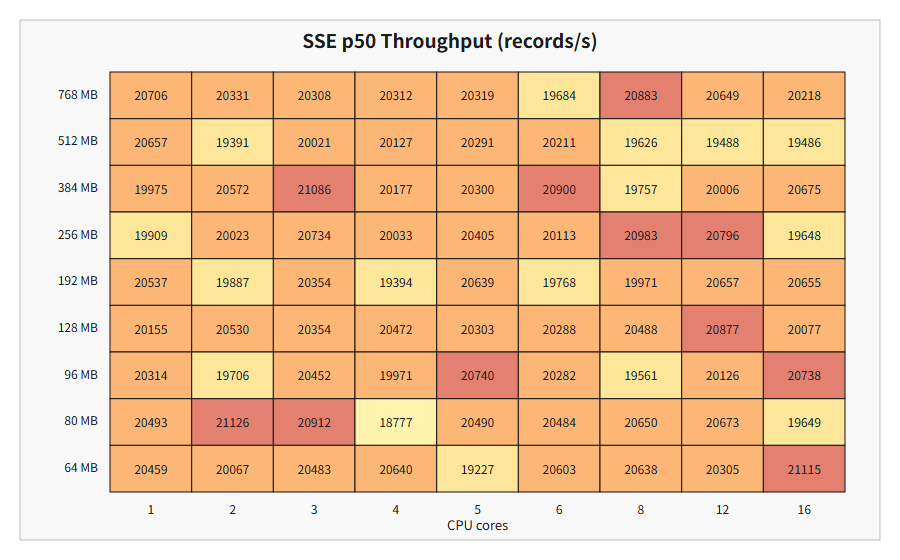
\includegraphics[width=0.92\textwidth]{sse_resource_heatmap_white.png}
  \caption{SSE 在不同 CPU 和内存配置下的 p50 吞吐量}
  \label{fig:sse-resource-heatmap}
\end{figure}

从热力图可以看出，在本次资源矩阵中，SSE 的吞吐量主要分布在
19,000 至 21,000 records/s 之间。不同资源配置之间虽然存在一定波动，
但整体差异较小，并未随着 CPU 核数或内存容量的增加而呈现持续上升趋势。
例如，部分较低资源配置下的吞吐量与高资源配置接近，个别配置甚至高于
对应的多核配置。

\begin{figure}[H]
  \centering
  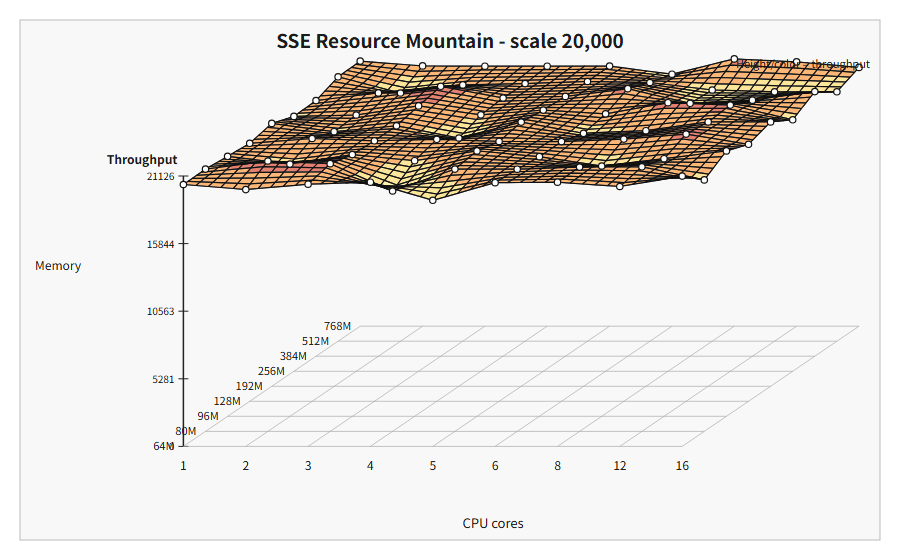
\includegraphics[width=0.92\textwidth]{sse_resource_mountain_white.png}
  \caption{SSE 吞吐量资源曲面}
  \label{fig:sse-resource-mountain}
\end{figure}

资源曲面整体较为平缓，进一步说明在当前 20,000 条记录规模下，SSE
候选筛选对 CPU 核数和内存容量的敏感程度相对较低。CPU 核数从 1 核增加到
16 核并未表现出稳定的线性加速，内存从 64 MB 增加到 768 MB 也没有带来
显著且持续的吞吐提升。

出现这一现象的原因可能在于，当前 SSE Export 路径除密码学计算外，还包含
记录读取、候选匹配、字段处理和结果写出等步骤。其中部分过程以串行方式执行，
并受到固定流程开销和输入输出操作的影响。因此，当任务规模相对有限时，单纯
增加 CPU 核数和内存容量并不能显著缩短执行时间。

本次测试中，SSE 在 64 MB 等较低内存限制下仍能够完成任务，表明其资源需求
相对较轻。结合吞吐量分布可以认为，SSE 适合作为隐私计算主链路中的前置候选
筛选服务。但是，该结论仅适用于当前测试规模，数据量、索引规模和并发请求数
进一步增加后，仍需重新评估其内存占用和吞吐变化。

\subsection{PJC 资源配置实验}

PJC 资源实验固定双方输入规模为 $1{,}000\times1{,}000$，分别调整 CPU
核数和内存限制，并记录任务能否完成以及成功运行时的 p50 吞吐量。与 SSE
相比，PJC 需要执行可交换加密、同态聚合以及 Server/Client 之间的协议交互，
其计算过程更复杂，预计对运行资源也更加敏感。

图~\ref{fig:pjc-resource-heatmap} 展示了各资源组合的运行状态和吞吐量。
图中的黑色区域表示该配置下任务未成功完成；单元格中带百分比的数据表示该
资源配置未能在所有重复实验中稳定成功。例如，\texttt{50 (75\%)} 表示该
配置的实验成功率为 75\%，成功样本的 p50 吞吐量为 50 items/s。

\begin{figure}[H]
  \centering
  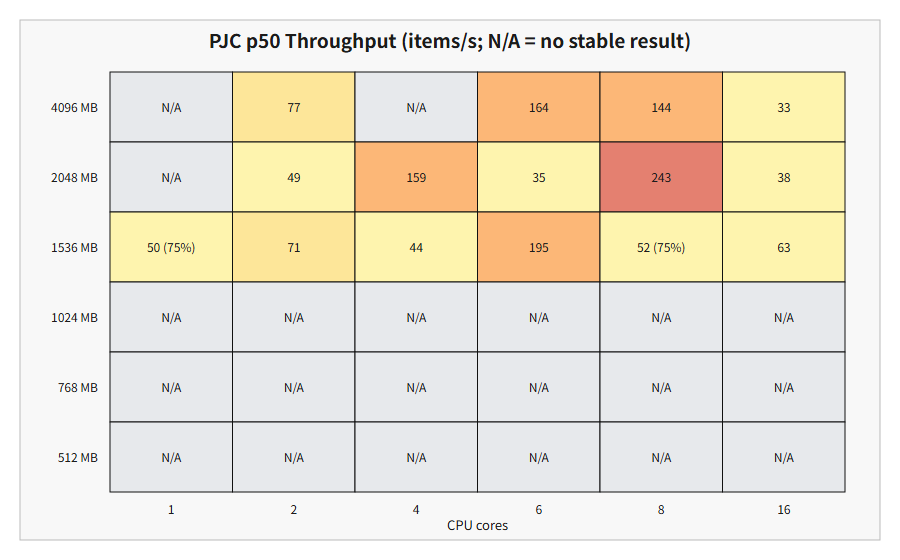
\includegraphics[width=0.92\textwidth]{pjc_resource_heatmap_white.png}
  \caption{PJC 在不同 CPU 和内存配置下的 p50 吞吐量}
  \label{fig:pjc-resource-heatmap}
\end{figure}

从结果可以看出，PJC 存在较为明显的内存运行边界。在 512 MB、768 MB 和
1024 MB 内存限制下，所有 CPU 配置均未能成功完成任务。当内存提高至
1536 MB 后，各 CPU 配置开始能够运行，但部分配置的成功率仍只有 75\%，
表明此时任务已经进入可运行区域，却尚未达到完全稳定的状态。

当内存提高至 2048 MB 和 4096 MB 后，成功运行的资源组合进一步增加，
说明增大内存能够显著改善 PJC 的可运行性。不过，较高内存并不能保证所有
CPU 配置均成功。例如，在 4096 MB 内存下，1 核和 4 核配置仍出现失败，
表明任务成功率还会受到进程调度、协议交互和运行时状态等因素影响，不能仅用
内存容量解释。

\begin{figure}[H]
  \centering
  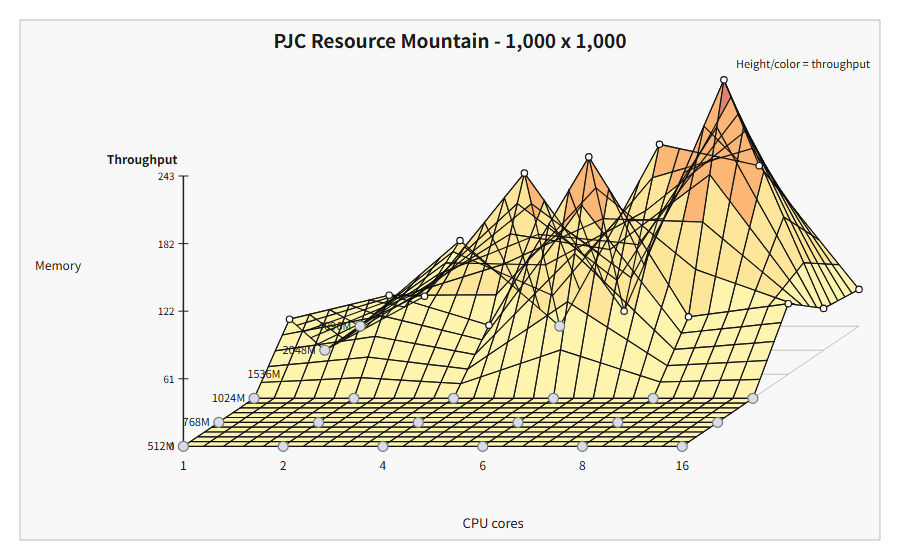
\includegraphics[width=0.92\textwidth]{pjc_resource_mountain_white.png}
  \caption{PJC 吞吐量资源曲面}
  \label{fig:pjc-resource-mountain}
\end{figure}

PJC 资源曲面具有明显的峰谷变化，与 SSE 的平缓曲面形成鲜明对比。在成功
运行的配置中，吞吐量大致分布在 33 至 243 items/s 之间，最高值出现在
2048 MB、8 核配置附近，达到约 243 items/s。但吞吐量并未随 CPU 核数
增加而单调上升。例如，某些 6 核或 8 核配置的吞吐量高于 16 核配置，
部分高内存组合的性能也低于较低内存组合。

这说明 PJC 的运行效率并不是由单一资源决定的。其性能同时受到密码学运算、
内存分配、Server/Client 进程调度、gRPC 通信、密钥生成和系统资源竞争等
因素影响。增加 CPU 核数可以提供更多计算资源，但如果实现中的并行度有限，
或者额外核心增加了调度和通信开销，实际吞吐量就不一定继续提高。

此外，部分成功配置的吞吐量较高，但重复实验的成功率没有达到 100\%。
因此，在选择部署参数时，不能只依据单次最高吞吐量，还应优先考虑任务成功率
和运行稳定性。

\subsection{资源特征对比}

SSE 和 PJC 的资源矩阵呈现出明显不同的性能特征。SSE 的吞吐量曲面较为
平缓，在本次测试范围内对 CPU 核数和内存容量的变化不敏感；PJC 则存在明显
的低内存失败区域，成功配置之间的吞吐量也具有较大波动。这一差异与两类模块
在系统中的职责和计算复杂度相符。

SSE 主要承担加密数据上的候选记录筛选。其处理流程相对轻量，能够在较低
内存配置下保持稳定运行，因此适合作为前置查询或候选筛选服务部署。Rust
Bridge 同样具有较高的数据准备吞吐量，可以在进入 PJC 之前快速完成标识
规范化、令牌化和输入文件生成。

相比之下，PJC 是主链路中计算和资源开销更明显的阶段。即使在
$1{,}000\times1{,}000$ 的输入规模下，低内存配置也可能导致任务失败；
在百万级输入测试中，其运行时间和峰值内存又会进一步增加。因此，实际部署
时不宜将 PJC 与轻量查询接口共享完全相同的资源池。

结合本次实验结果，后续部署可以采用差异化资源配置策略：SSE 作为相对轻量的
候选筛选服务进行常规调度；Record Recovery 根据候选规模设置单请求行数和
并发限制；PJC 则运行在独立的计算节点或资源隔离 worker 中，并为任务设置
明确的 CPU 配额、内存下限、执行超时、取消和重试机制。




\chapter{创新性说明}

\section{创新性边界}

本项目必须避免不准确的创新表述。SSE、PJC、HMAC、AES-GCM、PBKDF2、OIDC、OpenFGA 风格授权、数据净室和联邦学习框架都不是本项目首创。项目真正的创新点不在底层密码原语，而在系统组合、工程边界和治理闭环。

换句话说，本项目的贡献是将已有密码学和安全工程组件组织成一条具体的电商隐私分析链路，并在协议前后补充真实系统必须具备的权限、恢复、输入绑定、发布约束和审计证据。

\section{主链路组合创新}

传统 PJC 示例通常从双方准备好的 CSV 开始，直接运行交集计算。但真实场景下，数据并不会天然以安全 CSV 形式存在。我们的系统先用 SSE 在加密索引上筛选候选，再通过 record recovery 恢复最小必要字段，然后由 Bridge 生成 tokenized PJC 输入，最后才执行 PJC。

这种组合使每一阶段都有明确边界。SSE 限制候选，record recovery 限制明文字段，Bridge 限制标识表达，PJC 限制跨方计算，release gate 限制结果发布。它不是简单串联，而是分层收缩数据暴露面。

\section{输入治理创新}

很多隐私计算系统把输入准备视为外部问题。本项目没有这样做。Bridge 对 join key 做规范化和作用域 tokenization，生成 input commitment，并将 token secret 获取方式纳入 key agent 或 KMS adapter。这样，输入准备阶段也进入了审计和验证体系。

这种设计解决了一个现实问题：协议执行时可能没有泄露集合成员，但协议输入文件可能已经泄露原始标识，或者被替换成不真实数据。本项目通过 Bridge 和 input commitment 将这个薄弱点纳入主链路。

\section{发布治理创新}

PJC 算出结果并不意味着结果可以公开。项目通过 release gate、privacy budget、approval workflow、source attestation 和 external anchor 控制发布。它们的作用不是改变 PJC 协议，而是在协议外控制结果滥用。

这一点尤其适合电商分析场景。广告归因和复购分析很容易受到小交集和重复查询影响，因此系统必须拒绝过细结果，限制近似查询，记录审批责任，并为公开结果提供证据链。

\section{平台化创新}

项目不仅实现执行链路，还实现 metadata sidecar、query workflow、operator console、platform health、audit query API 和多类 benchmark。它使隐私计算从单次运行变成可管理平台：任务可以提交、审批、执行、查询、展示和归档。

这种平台化能力是本项目相较普通课程 demo 的主要优势。评委可以检查代码、运行命令、查看证据、观察控制台，也可以看到项目对安全边界的诚实描述。

\section{与已有工作的比较}

Google Private Join and Compute 与 SSEPy 分别代表了本项目所使用的两类基础能力。Google PJC 关注两方数据之间的隐私交集计算，可以在不公开具体交集成员的情况下得到交集规模和交集值之和；SSEPy 则面向可搜索对称加密方案的实现，使用户能够在加密索引上完成关键词检索。二者均为本项目提供了重要的技术基础，但各自主要解决隐私计算链路中的一个局部问题，并不直接覆盖数据进入计算之前的恢复控制、计算完成之后的结果治理以及跨阶段证据验证等环节\cite{googlepjc,ssepy}。

本项目并未重新设计 SSE 或 PJC 的底层密码学协议，而是围绕电商隐私分析场景，将密文候选筛选、受控记录恢复、关联标识处理、隐私交集计算和结果发布组织为一条连续链路。SSEPy 提供的密文检索能力被用于缩小候选数据范围，Google PJC 被用于完成两方交集统计和交集值聚合，在两者之间增加的 Record Recovery 与 Rust Bridge 则负责限制明文字段恢复，并将原始 join key 转换为作用域 HMAC token。PJC 输出之后，系统还通过 Release Gate、隐私预算、审批流程和审计证据控制结果的实际使用。

\begin{longtable}{p{0.21\textwidth}p{0.21\textwidth}p{0.21\textwidth}p{0.27\textwidth}}
\caption{本项目与 Google PJC、SSEPy 的能力比较}
\label{tab:existing-work-comparison}\\
\toprule
\textbf{对比维度} &
\textbf{Google PJC} &
\textbf{SSEPy} &
\textbf{本项目完整平台} \\
\midrule
\endfirsthead

\toprule
\textbf{对比维度} &
\textbf{Google PJC} &
\textbf{SSEPy} &
\textbf{本项目完整平台} \\
\midrule
\endhead

\bottomrule
\endfoot

主要定位 &
两方隐私交集统计与交集值聚合 &
可搜索对称加密方案实现与密文关键词检索 &
面向电商数据协作的端到端隐私分析链路 \\

密文候选筛选 &
未作为协议目标 &
支持加密索引和关键词搜索 &
将 SSE 查询作为 PJC 前的候选筛选阶段 \\

交集统计与聚合 &
支持交集规模和交集值之和计算 &
不属于其主要功能 &
接入 Google PJC 完成跨方交集统计与聚合 \\

候选记录恢复 &
要求调用方准备协议输入 &
主要关注密文检索过程 &
通过独立 Recovery Service 恢复最小必要字段 \\

原始标识处理 &
输入标识由协议调用方准备 &
检索词和索引由 SSE 方案处理 &
对 join key 进行规范化并生成作用域 HMAC token \\

输入与作业绑定 &
未提供完整的平台级作业绑定链路 &
未覆盖后续跨方计算作业 &
通过 job metadata、文件摘要和 input commitment 绑定输入 \\

结果发布控制 &
协议完成后输出交集规模和交集和 &
返回关键词检索结果 &
通过阈值、隐私预算、审批和 Release Gate 决定是否发布 \\

审计与证据验证 &
主要保留协议运行结果 &
提供方案运行和检索所需的基础日志 &
生成跨阶段结构化审计、Audit Chain 和 Audit Seal \\

任务管理与展示 &
未提供独立的平台控制面 &
提供基础客户端和服务端运行方式 &
提供 Metadata Sidecar、Query Workflow、Dashboard 和 Console \\

完整业务链路 &
需要由调用方在协议外自行组织 &
需要与其他业务模块组合 &
覆盖查询提交、候选筛选、恢复、计算、发布和审计过程 \\

\end{longtable}



Google PJC 的协议输出能够满足交集统计和聚合计算需求，但计算结果本身仍可能因交集规模过小、关联值异常或多次相关查询而产生推断风险。为此，本项目将协议计算结果继续交由发布治理模块处理，根据最小交集阈值、隐私预算、查询历史和审批状态决定是否生成公开报告。

在工程验证方面，本项目使用输入承诺、作业元数据和文件摘要连接不同处理阶段，并将 SSE Export、Record Recovery、Bridge、PJC 和 Policy Release 产生的记录汇总为审计链。与只保留单次搜索结果或协议计算结果相比，这种方式能够进一步说明任务由谁发起、使用了哪些输入、经过了哪些策略判断，以及最终结果为何被允许或拒绝发布。

因此，相较于已有基础项目的特点，本项目将原本分散的密文检索和隐私交集计算能力组织为可运行、可治理的平台链路。Google PJC 和 SSEPy 分别构成计算与检索基础，本项目在此之上补充了最小字段恢复、标识隔离、输入绑定、发布控制、任务管理和审计验证，使这些密码学能力能够更完整地服务于实际的跨方数据分析过程。



\chapter{不足与改进方向}

\section{当前不足}

第一，PJC 仍是半诚实参与方模型。当前系统能发现 repo-side 路径中的输入替换和无证据发布，但不能阻止恶意参与方主动偏离协议或提交伪造数据。

第二，SSE 仍有访问模式和搜索模式泄露。项目通过策略和审计降低滥用风险，但没有从协议层彻底隐藏访问模式。

第三，PJC 性能仍是大规模部署瓶颈。百万级双方输入已经通过流式路径完成，但耗时较长，资源敏感性明显，需要进一步分桶、并行、资源隔离和连接优化。

第四，真实生产信任根不是代码仓库可以完全替代的。OIDC、OpenFGA、Vault、cloud KMS、S3 Object Lock、Rekor、PostgreSQL HA 和 SRE 值守都需要在真实环境长期运行。

第五，电商事实层仍是适配基线。当前系统能承载订单、支付、履约、客服等基础语义，但还不是完整 customer 360 数据底座。

\section{后续改进}

在保持现有主线的前提下，后续可以先做工程增强：将 workflow worker 接入真实队列和 PostgreSQL，完善失败重试和状态恢复；将 PJC 放入资源隔离 worker，配合超时控制、分桶分片和任务调度；将审计锚点接入真实不可变存储或透明日志；将 operator console 与真实 OIDC 登录和角色授权联动。

如果要进一步提高安全等级，需要替换或增强底层协议。PJC 可以考虑 malicious-secure PSI-SUM、主动安全 MPC/2PC、零知识范围证明或可信执行环境；SSE 可以考虑 forward-private SSE、ORAM 或 OPRF-blinded query；发布治理可以引入更形式化的 differential privacy 机制，而不是只依赖启发式隐私预算。

\chapter{总结}

本项目围绕电商隐私分析中的跨方集合匹配和聚合计算问题，完成了一个由控制面数据库、SSE、受控记录恢复、Rust Bridge、Google PJC 和发布治理组成的平台工程。系统不仅能够算出交集数量和交集金额，还能说明这次计算是谁发起的、基于什么数据、经过哪些阶段、产生哪些证据、为什么允许或拒绝发布。

从完成度看，项目已经跑通主链路，完成控制面、工作流、操作台、发布门控、审计链、负向安全测试和性能 benchmark。标准示例结果正确，百万级 Bridge 和流式 PJC 测试完成，16 个顶层 verifier-facing 模块达到 repo-side 与 live-side ok。项目已经超过单一算法 demo，形成了竞赛阶段可展示、可验证、可复核的平台基线。

从创新性看，项目没有夸大为底层密码协议原创，而是把创新点落在系统集成和工程治理上。它将 SSE 候选筛选、record recovery、Bridge tokenization、PJC 计算和 release governance 组合为一条具体业务链路，补齐了任务审批、输入绑定、隐私预算、审计证据和展示界面等落地环节。

从收获看，团队认识到隐私计算系统不能只依靠密码协议。真正的系统安全来自协议、工程边界、密钥管理、权限控制、发布治理和审计证据的共同作用。后续如果继续推进，应沿着恶意安全计算、SSE 泄露缓解、真实 trust root 和生产级运维证据四个方向深化。

\appendix

\chapter{需要补充或替换的图片}

为配合正式报告呈现，建议补充或替换以下图片：

\begin{enumerate}
  \item \textbf{任务时序图：}展示从请求提交、审批、SSE、record recovery、Bridge、PJC 到 release gate 的全过程。
  \item \textbf{成果总览图：}展示主链路、控制面、安全治理、验证体系和操作台五类成果。
  \item \textbf{浅色 SSE 资源图：}替换当前红色背景热力图，突出吞吐稳定。
  \item \textbf{浅色 PJC 资源图：}替换当前黑色 FAIL 热力图，用浅灰斜线表示失败区域。
  \item \textbf{操作台截图：}至少补充 jobs、requests、audit/security 三类页面截图。
\end{enumerate}

\chapter{主要验证命令}

\begin{lstlisting}[language=bash]
# 端到端主链路
bash scripts/run_live_sse_bridge_demo.sh

# JSON 契约与 CI smoke
bash scripts/check_json_contracts.sh
bash scripts/check_ci_smoke.sh
python3 scripts/check_schema_backcompat.py

# 安全负向测试
python3 scripts/check_http_malformed_input_gate.py
python3 scripts/verify_audit_tamper_resistance.py --help

# Benchmark 入口
python3 scripts/benchmark_smoke.py --help
python3 scripts/benchmark_pjc.py --help
\end{lstlisting}

\begin{thebibliography}{99}

\bibitem{curtmola2006sse}
R. Curtmola, J. Garay, S. Kamara, and R. Ostrovsky.
Searchable Symmetric Encryption: Improved Definitions and Efficient Constructions.
In \textit{ACM CCS}, 2006.

\bibitem{cash2014dynamic}
D. Cash, J. Jaeger, S. Jarecki, C. Jutla, H. Krawczyk, M.-C. Rosu, and M. Steiner.
Dynamic Searchable Encryption in Very-Large Databases: Data Structures and Implementation.
In \textit{NDSS}, 2014.

\bibitem{googlepjc}
Google.
Private Join and Compute.
\url{https://github.com/google/private-join-and-compute}.

\bibitem{wiredpjc}
L. Newman.
Google Turns to Retro Cryptography to Keep Data Sets Private.
\textit{Wired}, 2019.
\url{https://www.wired.com/story/google-private-join-compute-database-encryption/}.

\bibitem{awscleanrooms}
Amazon Web Services.
AWS Clean Rooms.
\url{https://aws.amazon.com/clean-rooms/}.

\bibitem{fate}
FederatedAI.
FATE: An Industrial Grade Federated Learning Framework.
\url{https://github.com/FederatedAI/FATE}.

\bibitem{secretflow}
SecretFlow.
SecretFlow: A Unified Framework for Privacy-Preserving Data Intelligence and Machine Learning.
\url{https://github.com/secretflow/secretflow}.

\bibitem{nistgcm}
M. Dworkin.
Recommendation for Block Cipher Modes of Operation: Galois/Counter Mode (GCM) and GMAC.
NIST Special Publication 800-38D, 2007.

\bibitem{rfc2104}
H. Krawczyk, M. Bellare, and R. Canetti.
HMAC: Keyed-Hashing for Message Authentication.
RFC 2104, 1997.

\bibitem{rfc8018}
K. Moriarty, B. Kaliski, and A. Rusch.
PKCS \#5: Password-Based Cryptography Specification Version 2.1.
RFC 8018, 2017.

\end{thebibliography}

\end{document}
